\documentclass[12pt, a4paper]{article}
\usepackage{babel}
\usepackage{cleveref}
\usepackage{graphicx}

% Setter mindre marginer for å få mer plass
\usepackage[margin=2.5cm]{geometry}

% Pakke for å ha figurer ved siden av tekst
\usepackage{wrapfig}

% Pakke for å ha figurer side om side
\usepackage{subcaption}

\usepackage{tikz}
\usetikzlibrary{calc,trees,positioning,arrows,chains,shapes.geometric,  decorations.pathreplacing,decorations.pathmorphing,shapes,  matrix,shapes.symbols}


% Kommando som gjør at bilder kan være i en mappe som heter "bilder"
\graphicspath{ {./bilder/} }

% Må ha for referanselista
\usepackage{url}

\title{
    Project \#5\\
    \large System Integration and Testing\\
}

\author{
    Stein Lysberg
}


\begin{document}
\tikzstyle{block} = [rectangle, draw, text width=8em, text centered, rounded      corners, minimum height=1.6em]


    \maketitle
    \tableofcontents

    \thispagestyle{empty}
    \addtocounter{page}{-1}
    \clearpage

    \section{Introduction}
        
        This report is the fifth in a series of five. It will look at use cases for the scanner, the system architecture,
        system integration and testing of the
        finished plastic scanner. As the plastic scanner finishes a scan, the results are sent to a computer via serial communication. In the computer,
        these reading are presented on the monitor via a graphical user interface. This user interface has the option to store data,
        which allows for the creation of a database of values for known materials. Using this database, the interface could compare any
        value to already known values, and have a guess at which material it is scanning.

        \subsection{Use cases}
        
        Because the plastic scanner requires a computer to present its output, it is not very portable. This report will show that it is also
        sensitive to changing environments. For this reason, a realistic use case for could be at a stationary sorting station for plastic waste, shielded from
        sunlight. For example the the back of a van during a beach cleaning, or at a makeshift sorting facility. It should also be noted that the
        scanner is not yet reliable to distingush between all types of plastic, but it could still be useful for coarse sorting.


        \begin{figure}[h!]
            \centering
            \vspace{10pt}
                \begin{tikzpicture}
                    [node distance=1.5cm,]
                   \node (n1) at (0,0) [block]  {Computer};
                   \node (n2) [block, below of=n1] {Debugger};
                   \node (n3) [block, below of=n2] {NRF52832};
                   \node (n4) [block, right = 1.4 cm of n3] {TLC5920F};
                   \node (n5) [block, left = 1.4 cm of n3] {NAU7802};
                   \node (n6) [block, above of=n4] {LEDs};
                   \node (n7) [block, above of=n5] {Photodiode};

                   % Connectors
                   \draw [->] (n1) -- (n2)node[midway, right] {SWD};
                   \draw [->] (n2) -- (n3)node[midway, right] {SWD};
                   \draw [->] (n3) -- (n4)node[midway, above] {I$^2$C};
                   \draw [->] (n3) -- (n5)node[midway, above] {I$^2$C};
                   \draw [->] (n4) -- (n6)node[midway, right] {$v$};

                   \draw [->] (n2) -- (n1)node[midway, left] {UART};
                   \draw [->] (n3) -- (n2);
                   \draw [->] (n4) -- (n3);
                   \draw [->] (n5) -- (n3);
                   \draw [->] (n7) -- (n5)node[midway, right] {$v$};
                   \end{tikzpicture}
            \caption{System architecture}
            \vspace{-15pt}
            \label{fig:systemarchitecture}
        \end{figure}

        \subsection{System architecture}

        \begin{wrapfigure}[13]{r}{0.4\textwidth}
            \centering
            \vspace{-40pt}
                \begin{tikzpicture}
                    [node distance=0.8cm,
                    start chain=going below,]
                   \node (n1) at (0,0) [block]  {Power on};
                   \node (n2) [block, below of=n1] {LED-driver setup};
                   \node (n3) [block, below of=n2] {ADC setup};
                   \node (n4) [block, below of=n3] {ADC calibration};
                   \node (n5) [block, below of=n4] {LED on};
                   \node (n6) [block, below of=n5] {Read ADC};
                   \node (n7) [block, below of=n6] {LED off};
                   \node (n8) [block, below of=n7] {Print results};
                   % Connectors
                   \draw [->] (n1) -- (n2);
                   \draw [->] (n2) -- (n3);
                   \draw [->] (n3) -- (n4);
                   \draw [->] (n4) -- (n5);
                   \draw [->] (n5) -- (n6);
                   \draw [->] (n6) -- (n7);
                   \draw [->] (n6) -- (n7);
                   \draw [->] (n7) -- (n8);
                   \draw [->] (n8.west) -| ++(-0.4,0) |- (n5.west);
                   \draw [->] (n7.east) -| ++(0.4,0) |- (n5.east)node[midway, right] {5x};
                   \end{tikzpicture}
            \caption{Workflow chart}
            \label{fig:workflow}
        \end{wrapfigure}

        Reports 3 and 4 discussed the use of the TLC5920F LED-driver and the NAU7802 ADC individually. This report will look at how they work together
        as part of the system. \Cref{fig:systemarchitecture} shows the system architecture. The computer programs the NRF52832 microcontroller
        using Serial Wire Debug protocol, via the debugger on the development kit. The debugger is also a NRF52832, but in this application it only handles
        interfacing with the computer. The microcontroller controls both the ADC and the LED-driver using I$^2$C.
        Led LED-driver supplies voltage to the LEDs.  The ADC reads a voltage from the photodiode.

        \Cref{fig:workflow} shows the flow of the code in this project. After power-up, the microcontroller checks that it can communicate with the LED-driver.
        it then configures the LED-driver by writing the appropriate values to its registers. The process is repeated for the ADC, which is also
        prompted to do its own internal calibration routine. Following this, the code loops through the LEDs by turning them on, reading from
        the ADC, and turning them off again. After all six LEDs have been looped over, the results from the six scans are printed to the console.

        \section{Testing}

            \begin{wrapfigure}[12]{r}{0.45\textwidth}
                \centering
                \vspace{-40pt}
                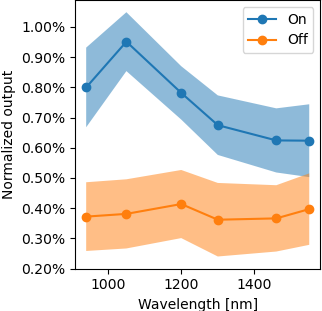
\includegraphics[width=0.4\textwidth]{LED_readings.png}
                \caption{Effect of LEDs.}
                \label{fig:LED_readings}
            \end{wrapfigure}

            Tests have been conducted by performing scans of various
            items and environments, and then storing and analyzing the results.
            These tests will be explained in the following section. The lines on the graphs
            are the averages of a series consisting of between 20 and 100 readings. The shaded areas around the lines
            are the averages plus/minus one standard deviation. The $x$-axis represent the wavelength of the LED
            that is currently on, and the $y$-axis is normalized between the minimum and maximum values across
            all readings we have done.
            
            \subsection{Integration testing}
            
          
            \Cref{fig:LED_readings} shows the effect of the LEDs on the ADC. For this dataset the plastic scanner sat on a table
            making readings of the air, with the LEDs either on or off, and approximately 100 readings were taken in both cases.

            \subsection{Scanning in- and outdoors}

            \begin{wrapfigure}[11]{r}{0.45\textwidth}
                \centering
                \vspace{-20pt}
                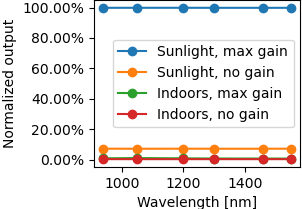
\includegraphics[width=0.40\textwidth]{gain_readings.png}
                \caption{Effect of sunlight and gain.}
                \label{fig:gain_readings}
            \end{wrapfigure}

            \Cref{fig:gain_readings} shows the effects of gain on the readings, as well as the effect
            of environmental light. The tests were conducted indoors and outdoors, using the maximum gain for the ADC, which is 128,
            and the minimum which is 0. The indoors tests were conducted in a room with the lights on
            and the curtains closed, and the outdoors tests were conducted in the window sill of the same
            room, where the photodiode sensor was exposed to the sun. In this scale, the bottom two sets of
            readings (indoors with and without gain) are almost indistinguishable. 70-100 readings were taken for each line.
            This graph also has a shaded area representing plus/minus one standard deviation, like \cref{fig:LED_readings}, but the scale is so large that they are indistinguishable
            from the lines.

            \subsection{Scanning production pellets}

            \begin{figure}[h!]
                \centering
                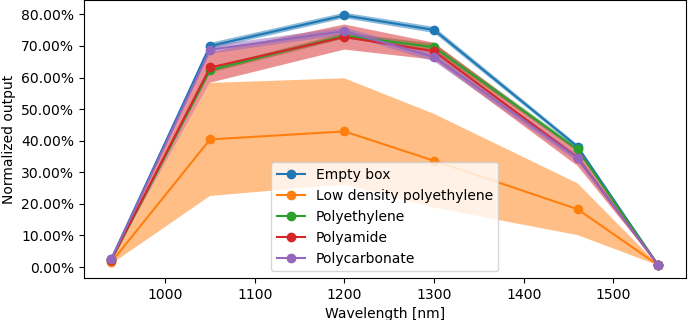
\includegraphics[width=\textwidth]{multiple_materials.png}
                \caption{Scans of various production pellets.}
                \label{fig:plastics}
            \end{figure}

            \noindent \Cref{fig:plastics} shows the results of some scans of plastic production pellets in a small box with
            mirrored walls. In this experiment the box sat on the table, was filled with pellets, and the plastic scanner was
            held over it to scan into the box. The top line is the box with mirrored walls, without contents, so as to reflect as much light as
            possible, included for reference. 20-30 readings were taken for each material.
            
            \subsection{Scanning items}
            In addition to scanning environments and pellets, a few items were scanned to see how the scanner distinguishes between them. Namely,
            a polyester cap and a 3D-printed PLA keychain. As \cref{fig:capkeycombo} shows, the dinstinction is clear, showing that the plastic scanner
            can make clear distinctions between different objects in the same environment. 30 readings were taken for the cap, and 50 for the keychain.


            \begin{figure}[h!]
                \begin{subfigure}[t]{0.25\textwidth}
                    \centering
                    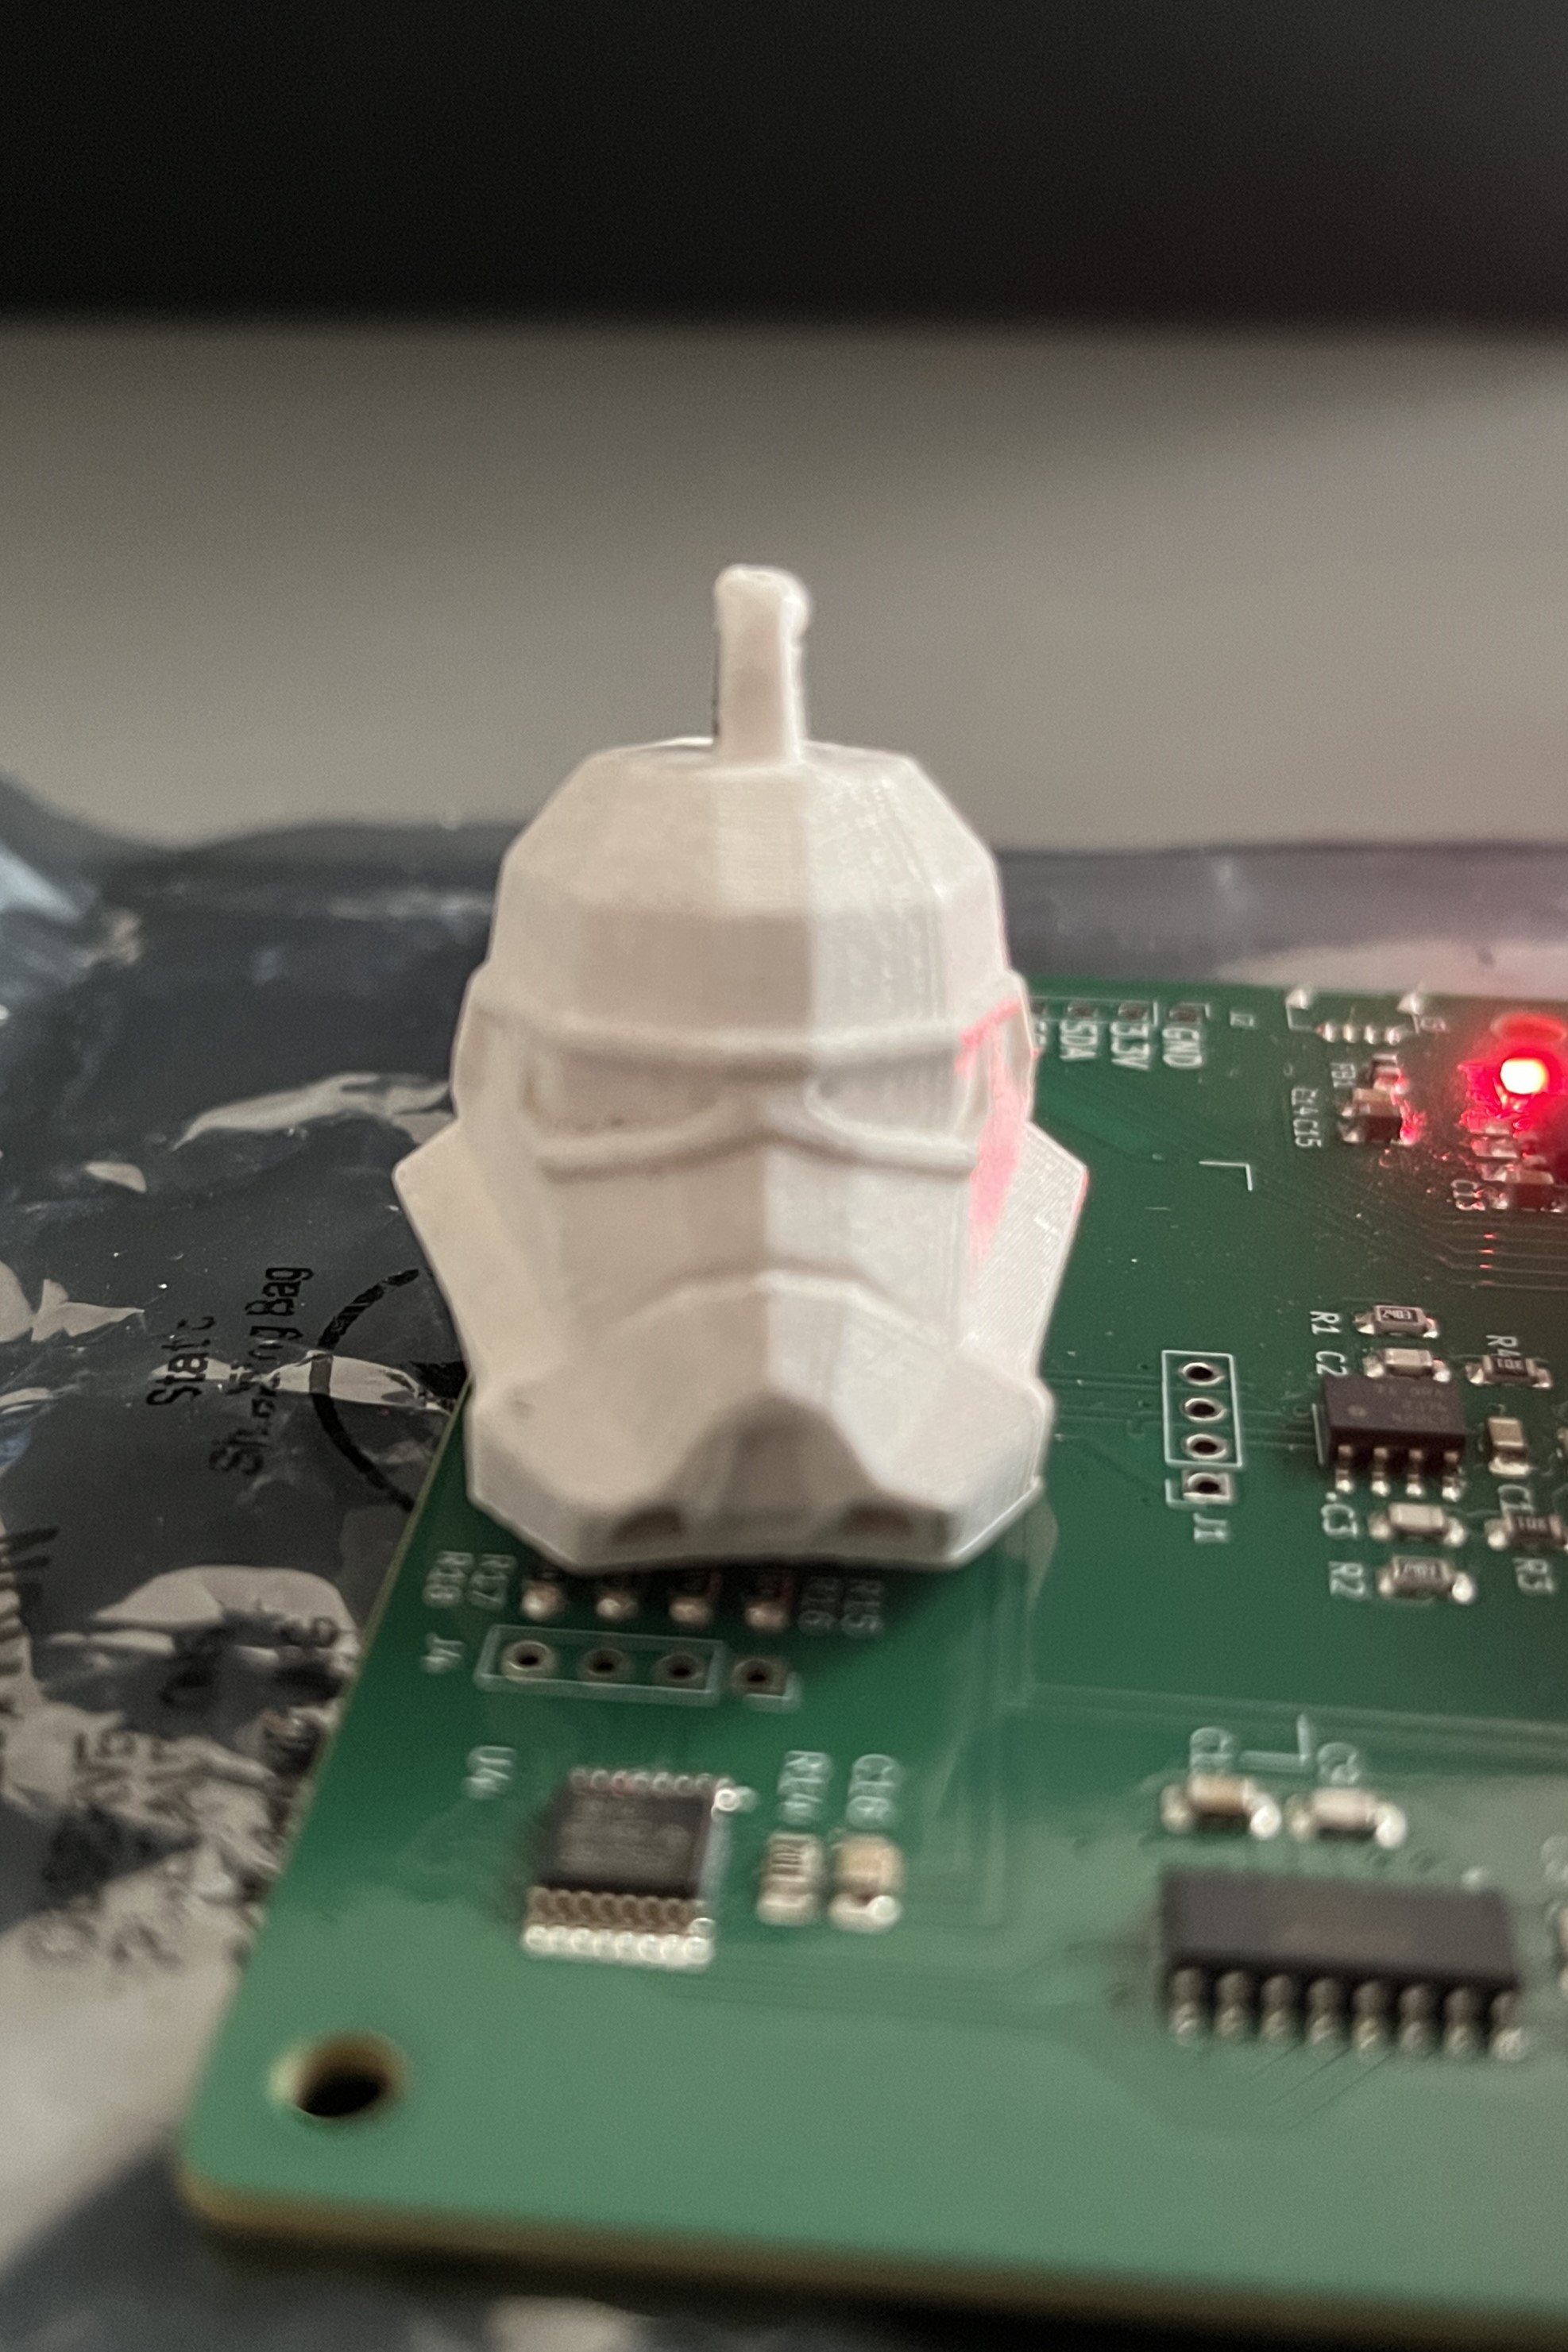
\includegraphics[width=0.8\textwidth]{Key.JPG}
                    \label{fig:key}
                    \caption{Keychain.}
                \end{subfigure}%
                \begin{subfigure}[t]{0.25\textwidth}
                    \centering
                    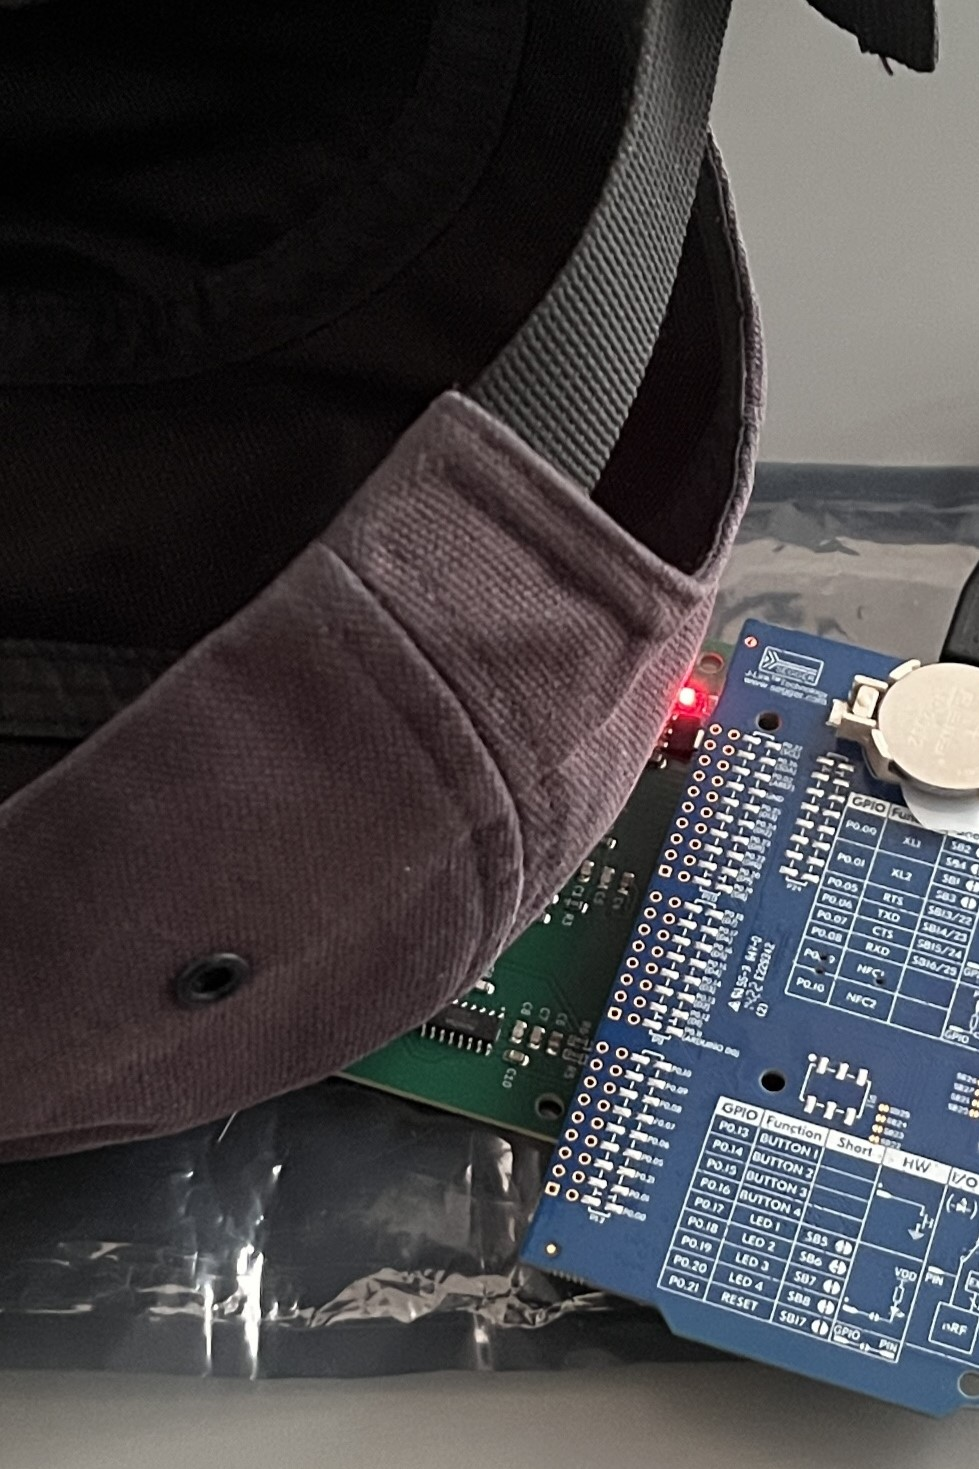
\includegraphics[width=0.8\textwidth]{Cap.JPG}
                    \label{fig:cap}
                    \caption{Cap.}
                \end{subfigure}%
                \begin{subfigure}[t]{0.5\textwidth}
                    \centering
                    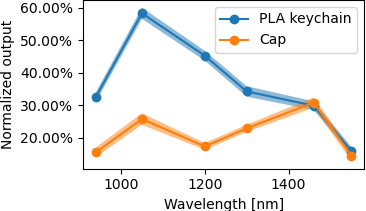
\includegraphics[width=\textwidth]{capkey.png}
                    \label{fig:capkey}
                    \caption{Spectra.}
                \end{subfigure}
                \caption{A cap, a keychain, and their spectra.}
                \label{fig:capkeycombo}
                \vspace{0pt}
            \end{figure}
    \clearpage
    \section{Discussion}
        This section will discuss the results from the tests, as well as suggest some ways to further improve
        upon the current state of the plastic scanner.

        \subsection{Test results}
            
            \subsubsection{Integration}
                As shown in \cref{fig:LED_readings}, the LEDs being on affect the values from the ADC, which
                indicates that these components work together as they should. Since these reading were
                taken without an object in front of the scanner, these results also show that the photodiode sensor
                picks up some light directly from the LEDs.
            \subsubsection{Environments}
                \Cref{fig:gain_readings} showed the effect of gain on the values produced by the ADC, as well as the
                environment light. The scan of sunlight shows all readings close to 100\%, which means they are the highest
                readings recorded in any of the tests, because the scale is normalized between lowest and highest recorded value across all tests.
                It is worth noting that a scan in the sunlight with no gain yields higher readings than an indoor scan with maximum gain.

            \subsubsection{Materials and items}
                \begin{wrapfigure}[11]{r}{0.55\textwidth}
                    \centering
                    \vspace{-45pt}
                    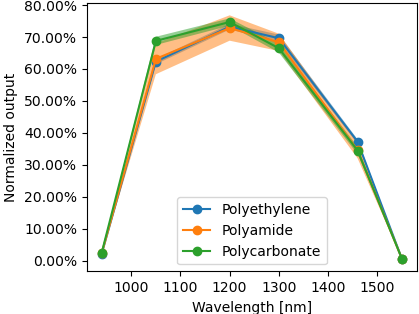
\includegraphics[width=0.45\textwidth]{pe_pa_pc.png}
                    \caption{Excerpt from \cref{fig:plastics}.}
                    \label{fig:pe_pa_pc}
                \end{wrapfigure}

                \Cref{fig:plastics}, the results of scans of production pellets made of various plastics, shows that different items
                yield different readings. The empty box is easily distinguishable from low density polyethylene, but regular polyethylene,
                polyamide and \linebreak polycarbonate look about the same. as shown in \cref{fig:pe_pa_pc}. The cap and keychain in
                \cref{fig:capkeycombo} shows that the scanner has the potential to clearly distinguish different items, but it is unclear
                whether this is because they are made from different plastics, or because they differ in some other way, like coloring or density.

            \subsubsection{Issues and sources of error}
                Not being able to distinguish between polyethylene, polyamide and polycarbonate, as shown in \cref{fig:plastics}, is a problem. The cause for this could be
                that the box was not sufficiently full, so the readings were more affected by the mirrors than the pellets. This could also why these curves are
                so close to that of the empty box. \par
                Another source of error in this experiment is that the environment may not have been the same in all tests. The plastic scanner was
                held manually as the scan was conducted, so alignment and spacing with the box may not have been the same for all readings. This
                is especially noteworthy in the case of low density polyethylene, where the standard deviation is greatest.

        \subsection{Potential improvements}
                Although no more work will be done on the plastic scanner, a few potential improvements to it will be suggested in the following
                section. They are separated into potential software and hardware improvements.

        \subsubsection{Software improvements}
            
            The suggested improvement or using interrupts rather than polling for the ADC was discussed in report 4. This suggestion will build on that.
            The code for the plastic scanner loops continuously, starting the next scan cycle immediately after printing the previous. Instead of doing this,
            a scan cycle (or a number of scan cycles) could be triggered by a button connected to the GPIO of the nRF52. If this was implemented, the nRF52,
            TLC5920F and NAU7802 could all be set to low-power mode between the scans. This improvement would be most relevant if this was to be used as a
            handheld device. This could be similar to the command line interface implementation in the Arduino code \cite{arduinocode}.\par
            \begin{wrapfigure}[11]{r}{0.4\textwidth}
                \centering
                \vspace{-0pt}
                    \begin{tikzpicture}
                        [node distance=0.8cm,
                        start chain=going below,]
                       \node (n1) at (0,0) [block]  {Trigger};
                       \node (n2) [block, below of=n1] {Make a scan};
                       \node (n3) [block, below of=n2] {Evaluate result};
                       \node (n4) [block, below of=n3] {Adjust gain};
                       \node (n5) [block, below of=n4] {Calibrate ADC};
                       \node (n6) [block, below of=n5] {End};

                       % Connectors
                       \draw [->] (n1) -- (n2);
                       \draw [->] (n2) -- (n3);
                       \draw [->] (n3) -- (n4);
                       \draw [->] (n4) -- (n5);
                       \draw [->] (n5) -- (n6);
                       \draw [->] (n3.west) -| ++(-0.4,0) |- (n6.west);
                       \draw [->] (n5.east) -| ++(0.4,0) |- (n2.east);
                       \end{tikzpicture}
                \caption{Gain calibration.}
                \label{fig:gaincalibration}
            \end{wrapfigure}
            As \cref{fig:gain_readings} shows, the readings vary a lot with the gain and environment lighting. A function could be added, also triggered by
            a switch connected to the GPIO, which sets an appropriate gain for the ADC. This would let readings be more similar across different environments.
            It could be implemented as shown in \cref{fig:gaincalibration}. Note that the ADC has to do its own calibration routine after setting a new gain \cite{nau}.
        
            \subsubsection{Hardware improvements}
            To increase the reliability of the scanner, more LEDs could be added for increased resolution. The LEDs currently on the PCB
            cover the full spectral range of the photodiode sensor, but there could be \textit{more} LEDs within this range, creating a finer
            resolution. The two idle LED slots on the PCB could be used for this. To further increase reliability, more and more leds and
            photodiodes with different wavelengths and spectral ranges can be added, but it should be kept to a minimum to make sense in the
            contect of this project.\par
            As \cref{fig:LED_readings} shows, the photodiode picks up some light directly from the LEDs. If this could be reduced, more of the
            collected light would be \textit{reflected} light, which is what is useful. This could be achieved by making a case for the plastic
            scanner, with a physical barrier between the LEDs and the photodiode. A case would also make the whole contraption less vulnerable,
            and nicer to handle.

    \section{Conclusions}

            This report has shown that although the plastic scanner in its current state produces appropriate results in the conditions
            it has been tested in, it is not yet fully reliable as a tool to distinguish between all different types of plastic. Although this project
            is finished, there are many improvements which can still be made. With more testing in different environments, and a database of known values for known materials,
            it may become easier to determine what type of plastic is being scanned. This may also require some knowledge of chemistry and data analysis
            which is beyond the scope of this
            report.

    \clearpage
    \addcontentsline{toc}{section}{References}  
    \bibliographystyle{IEEEtran}
    \bibliography{bibliography}

\end{document}